% This is based on "sig-alternate.tex" V1.9 April 2009
% This file should be compiled with V2.4 of "sig-alternate.cls" April 2009
%
\documentclass{report}

\usepackage[english]{babel}
\usepackage{graphicx}
\usepackage{tabularx}
\usepackage{subfigure}
\usepackage{enumitem}
\usepackage{url}

\usepackage{color}
\definecolor{orange}{rgb}{1,0.5,0}
\definecolor{lightgray}{rgb}{.9,.9,.9}
\definecolor{java_keyword}{rgb}{0.37, 0.08, 0.25}
\definecolor{java_string}{rgb}{0.06, 0.10, 0.98}
\definecolor{java_comment}{rgb}{0.12, 0.38, 0.18}
\definecolor{java_doc}{rgb}{0.25,0.35,0.75}

% code listings

\usepackage{listings}
\lstloadlanguages{Java}
\lstset{
	language=Java,
	basicstyle=\scriptsize\ttfamily,
	backgroundcolor=\color{lightgray},
	keywordstyle=\color{java_keyword}\bfseries,
	stringstyle=\color{java_string},
	commentstyle=\color{java_comment},
	morecomment=[s][\color{java_doc}]{/**}{*/},
	tabsize=2,
	showtabs=false,
	extendedchars=true,
	showstringspaces=false,
	showspaces=false,
	breaklines=true,
	numbers=left,
	numberstyle=\tiny,
	numbersep=6pt,
	xleftmargin=3pt,
	xrightmargin=3pt,
	framexleftmargin=3pt,
	framexrightmargin=3pt,
	captionpos=b
}

% Disable single lines at the start of a paragraph (Schusterjungen)

\clubpenalty = 10000

% Disable single lines at the end of a paragraph (Hurenkinder)

\widowpenalty = 10000
\displaywidowpenalty = 10000
 
% allows for colored, easy-to-find todos

\newcommand{\todo}[1]{\textsf{\textbf{\textcolor{orange}{[[#1]]}}}}

% consistent references: use these instead of \label and \ref

\newcommand{\lsec}[1]{\label{sec:#1}}
\newcommand{\lssec}[1]{\label{ssec:#1}}
\newcommand{\lfig}[1]{\label{fig:#1}}
\newcommand{\ltab}[1]{\label{tab:#1}}
\newcommand{\rsec}[1]{Section~\ref{sec:#1}}
\newcommand{\rssec}[1]{Section~\ref{ssec:#1}}
\newcommand{\rfig}[1]{Figure~\ref{fig:#1}}
\newcommand{\rtab}[1]{Table~\ref{tab:#1}}
\newcommand{\rlst}[1]{Listing~\ref{#1}}

% General information

\title{Distributed Systems -- Assignment 1}

% Use the \alignauthor commands to handle the names
% and affiliations for an 'aesthetic maximum' of six authors.

\numberofauthors{3} %  in this sample file, there are a *total*
% of EIGHT authors. SIX appear on the 'first-page' (for formatting
% reasons) and the remaining two appear in the \additionalauthors section.
%
\author{
% You can go ahead and credit any number of authors here,
% e.g. one 'row of three' or two rows (consisting of one row of three
% and a second row of one, two or three).
%
% The command \alignauthor (no curly braces needed) should
% precede each author name, affiliation/snail-mail address and
% e-mail address. Additionally, tag each line of
% affiliation/address with \affaddr, and tag the
% e-mail address with \email.
%
% 1st. author
\alignauthor Robin Guldener\\
	\affaddr{ETH ID 11-930-369}\\
	\email{robing@student.ethz.ch}
% 2nd. author
\alignauthor Nico Previtali\\
	\affaddr{ETH ID 11-926-433}\\
	\email{pnico@student.ethz.ch}
%% 3rd. author
\alignauthor Lukas Bischofberger\\
	\affaddr{ETH ID 11-915-907}\\
	\email{lukasbi@student.ethz.ch}
}


\begin{document}

\maketitle

\begin{abstract}
%Concisely state (i) which Android device you used, (ii) which tasks you completed and which are working correctly or limited, and (iii) what your specific enhancements are.

We developed two mobile applications for the Android platform from the ground up for the HTC Desire Nr. 25. We completed all of the tasks and our apps worked without crashes on the device. We also completed the enhancements in the following way: (1) After the device alarm has gone off, we start logging the path the thief walks. (2) For suppressing the alarm we created the possibility to save a friends phone number and continuously send GPS data to it. If no phone number is specified we try to acquire to phone's default email account and send the GPS data to this.

\end{abstract}

\section{Introduction}

For this assignment we implemented two mobile applications on the Android platform using the Android Developer Tools based on Eclipse\cite{androidDevTools}. For two out of three team members this was the first time working with Android and subesequently the majority of the time spent on the project was devoted to reading the Android API Guides\cite{androidAPIGuides} and Android Reference\cite{androidAPIReference}. Whilst the documentation material is mostly very well written, there are a few corner cases where different documents describe methods in mutual disagreement and the provided GUI editing tools of the Android Developer Tools have not always worked to our satisfaction.

Our team of three was split into two, with Lukas Bischofberger and Nico Previtali implementing the Anti-Theft Alarm and Robin Guldener implementing the Sensing with Android application. The reporting task was also split accordingly with Robin Guldener additionally covering the Introduction and Conclusion parts whilst Nico Previtali and Lukas Bischofberger also described their efforts for the enhancements of the Anti-Theft Alarm.

\section{Sensing with Android}
The Sensing with Android application (SwA) allows any Android device owner to quickly get an overview of all the sensors available on her device and to read raw data from any sensor in realtime. Additionally, SwA also enables the user to quickly explore the actuators of their device using the builtin Actuators Activity, which supports activating a device's builtin vibrator and playing a predefined, aurally pleasant jingle of bells.
\par
\indent
In the following paragraphs each Activity will be presented in detail.
\begin{figure}
    \centering
    \subfigure[MainActivity]{
        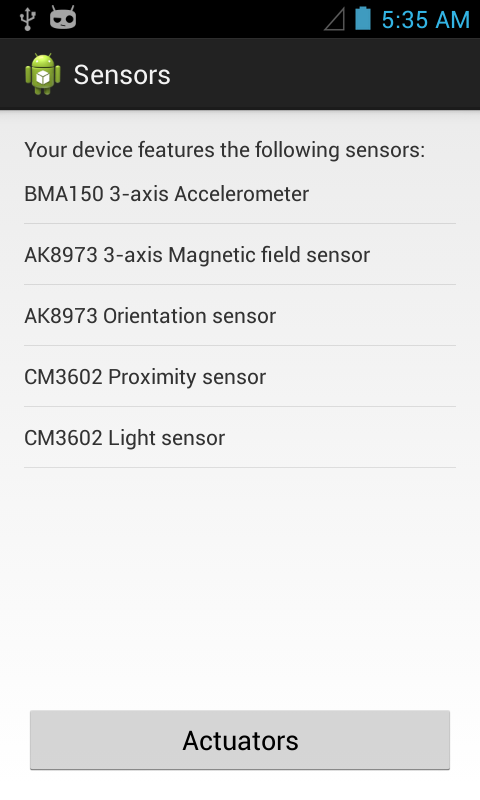
\includegraphics[height=4.2cm]{screen-sensors-main}
        \lfig{screenshot1}   
    }
    \hfill
    \subfigure[SensorsActivity]{
        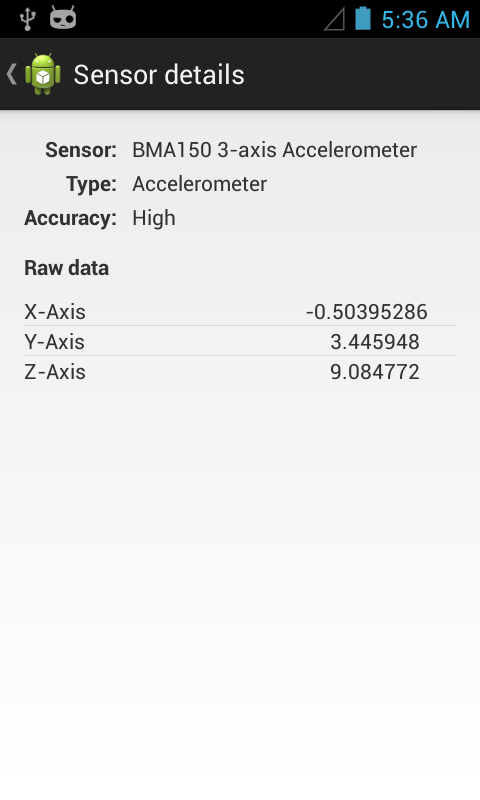
\includegraphics[height=4.2cm]{screen-sensors-details}
        \lfig{screenshot2}
    }
    \hfill
    \subfigure[ActuatorsActivity]{
        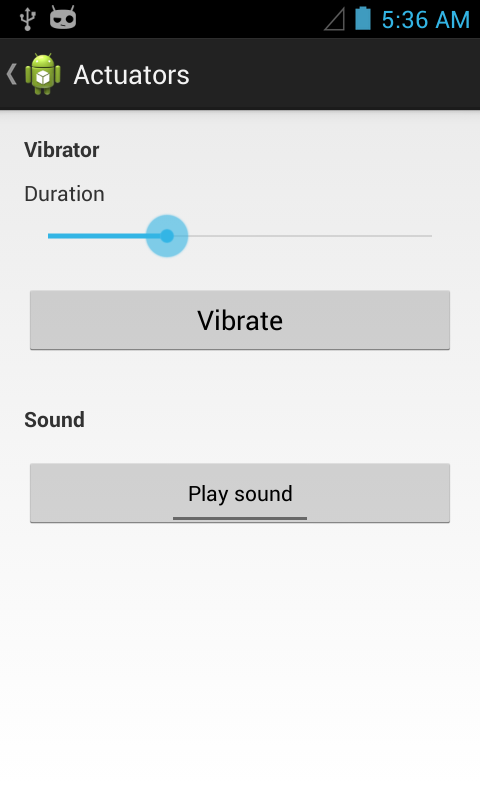
\includegraphics[height=4.2cm]{screen-sensors-actuators}
        \lfig{screenshot3}
    }
    \caption{Activities of the SwA application. Figure (a) shows an example of the sensors available on the lab-provided HTC desire. Figure (b) shows the readings for a particular time of the device's builtin accelerometer. Figure (c) displays the Actuators Activity.}
\end{figure}
\par
The Main Activity (cf. \rfig{screenshot1}) is the sole entry point of the Application and thus also the only activity that is listed in the launcher. It is the heart of the SwA application and displays a ListView containing all the names of the available sensors. This allows for the efficient selection of any particular sensor. To make the interaction with the list easier for humans with thicker fingers or any potential feline users, we have increased the height of a single row in the list beyond the default value. First tests have shown a particular increase in user-satisfaction, which we could directly link to this design decision.
\indent
One of the main challenges of the Main Activity is how to pass on the information which sensor was selected to the sensor details activity. We have resolved this issue by using the Java provided hashCode function\cite{javaHashCode} as detailed in \rlst{hashCode}. We consider this a particularly elegant solution as it does not depend on any, not necessarily unique, sensor names and leverages existing language design features.

\lstset{language=Java,caption={Passing the selected sensor using Java's hashCode method},label=hashCode} 
\begin{lstlisting}
// s holds a reference to the selected Sensor object
Intent intent = new Intent(this, SensorActivity.class);
intent.putExtra("sensor", s.hashCode());
this.startActivity(intent);
\end{lstlisting}

\par
\indent
The Sensors Activity (cf. \rfig{screenshot2}) provides detailed information on the selected sensor such as the sensor type and provides realtime access to both the raw sensor data as well as the current accuracy of the measured data. To populate the ListView displaying the raw data we have implemented a SensorAdapter, which is a sensor aware implementation of the abstract Adapter class that adjusts the data source exposed to the ListView to the particular sensor currently selected. This provides a clean solution to the heterogenous data we receive from the SensorEvent class\cite{androidSensorEvent} and allows for maximum compatability even with future sensor types.
\par
\indent
Finally the Actuators Activity (cf. \rfig{screenshot3}) employs a simplistic interface to allow the user to interact with the device's builtin vibrator and play a predefined sound file. The duration of the vibration can be conveniently adjusted using a SeekBar and allows vibration durations ranging from 0ms up to 1000ms, enabling the user to explore different kinds of tactile feedback in a minimal amount of time. Great care was also taken when choosing the builtin sound file and we finally settled on a pleasing, yet very well noticeable jingle of bells.

\section{The Anti-Theft Alarm}

The Anti-Theft Alarm application allows the user to secure their device against thiefs. In the application you can activate the sensor logic, which is then supervising if the device is moved within a certain amout of time. If the device is continiously moved within a set amount of time, the sensor logic triggers the alarm: A sound file is played at full volume and in the background the application starts to periodically send out GPS coordinates. The coordinates are either sent by SMS (if a recipient number was configured by the user) or alternatively by e-mail. All the necessary settings can comfortably be set in the application's settings, which are conveniently available from the main menu.

To detect when the device is stolen we used the accelerometer sensor to recognize movements. The accelerometer measures the acceleratoin of the device in the three dimensions of space. For each of the dimensions we measure the acceleration and compare them to some fixed threshold. This is necessary as the sensor is highly sensitive and registers even very small changes in acceleration but we only want to react to faster movements.

\lstset{language=Java,caption={Threshold the retrieved data to only detect wilful movements.},label=threshold} 
\begin{lstlisting}
float threshold = 0.2;
float x = event.values[0];
float y = event.values[1];
float z = event.values[2];

float diffX = Math.abs(Math.abs(oldX) - Math.abs(x));
float diffY = Math.abs(Math.abs(oldY) - Math.abs(y));
float diffZ = Math.abs(Math.abs(oldZ) - Math.abs(z));

// only issue when the the sensor values aren't within a certain threshold
if (diffX >= threshold || diffY >= threshold || diffZ >= threshold) {
	...
}
\end{lstlisting}

% \begin{figure}
%     \centering
%     \subfigure[Accelerometer]{
%         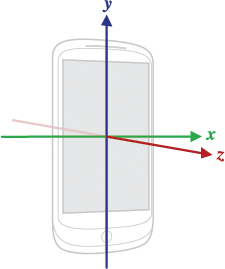
\includegraphics[height=4.2cm]{axis_device}
%         \lfig{axis}   
%     }
%     \caption{Accelerometer of the device.}
% \end{figure}

The main part of the sensor logic is the Anti-Theft service which runs in the background. This service registers the movements and triggers the alarm even if the application is closed or the device is locked. The service is started when clicking the ToggleButton in the Main Activity and stopped when disarming the device or deactivating the Anti-Theft application. Movements are recognized by the MovementDetector class. This class holds all the methods invoked by the system when the observed sensor has changed values. To avoid an alarm upon non-deliberate movements we defined a timestamp after a sensor change and waited for a second change within five seconds. Then if a third change at least five seconds after the first occurrence was detected, the alarm gets started. Obviously the user is able to disable the alarm for a self-specified amount of time after the detection.

\lstset{language=Java,caption={MovementDetector},label=MovementDetector} 
\begin{lstlisting}
// register accelerometer listener
movementDtr = new MovementDetector(this, this);
sensorManager.registerListener(movementDtr, accelerometer, SensorManager.SENSOR_DELAY_NORMAL);
\end{lstlisting}

\begin{figure}
    \centering
    \subfigure[PreferenceActivity]{
        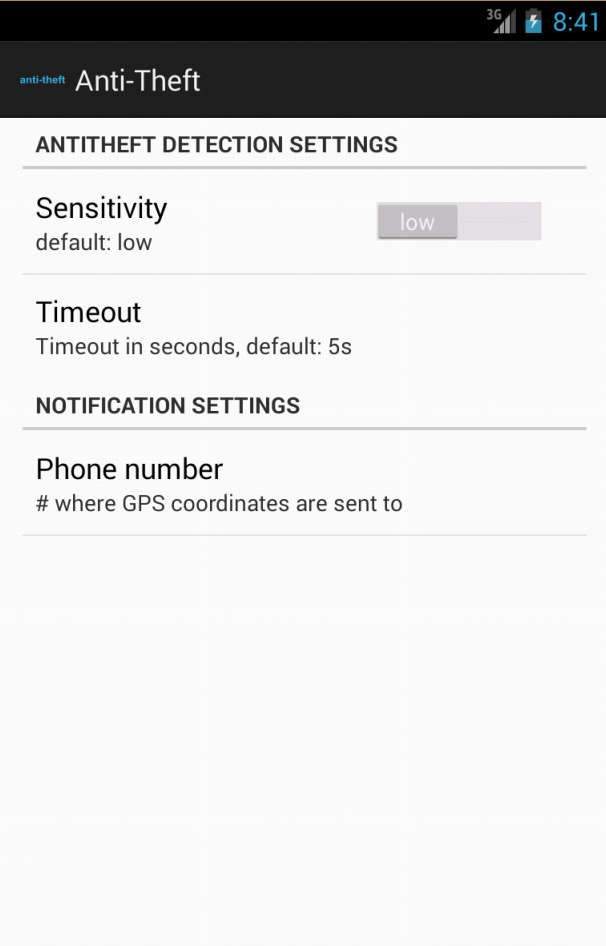
\includegraphics[height=6cm]{anti-theft-settings}
        \lfig{screenshot4}   
    }
    \hfill
    \subfigure[MainActivity]{
        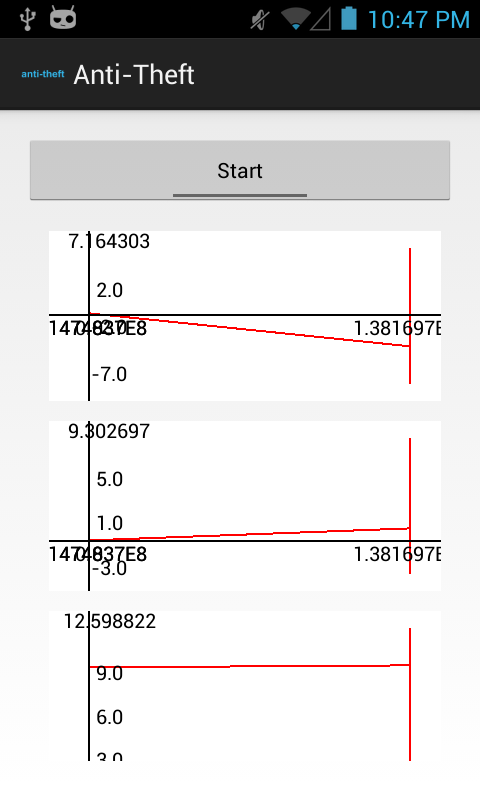
\includegraphics[height=6cm]{anti-theft-graph}
        \lfig{screenshot5}
    }
    \caption{Activities of the AT application. Figure (a) shows the preference activity where all settings are saved. Figure (b) shows the graph with the sensor data after an alarm has gone off.}
\end{figure}

The settings of the application are passed to the service by using the Android standard way of passing data between intents. This extra data is then retrieved by the service in the onStartCommand method. When the service triggers the alarm an ongoing notification is issued. This notification can not be cleared by the user. If the users clicks on it, it will forward him to the MainActivity where he can disarm the alarm.

\lstset{language=Java,caption={Passing data to the service},label=MovementDetector} 
\begin{lstlisting}
antitheft.putExtra("sensitivity", sharedPrefs.getBoolean("sensitivity", false));
antitheft.putExtra("timeout", sharedPrefs.getString("timeout", "5"));
antitheft.putExtra("number", sharedPrefs.getString("phone", null));
\end{lstlisting}

\section{Enhancements}

The application visualizes each dimension of the recorded data in three simple 2D plots. The x-axis is the time and the y-axis is the sensors dimension. Thus the first plot is the plot of the recorded sensor data in the X-dimenson, the second plot the one of the Y-dimension and the last one in the Z-dimension. To pass the data around the application we used a class instantiated with the Singleton design pattern. This class, called AccelDataSet stores all the recorded data. The plots are done using a class open source provided by Ankit Srivastava\cite{androidplot}. This is a simple class with takes arguments for the x and y axis and then plots the data with a curve.

\lstset{language=Java,caption={Using the plot2d class provided by Ankit Srivastava},label=plot2d} 
\begin{lstlisting}
plot2d graphX = new plot2d(this, time, xValues, 1);
plot2d graphY = new plot2d(this, time, yValues, 1);
plot2d graphZ = new plot2d(this, time, zValues, 1);
viewgroup.addView(graphX, params);
viewgroup.addView(graphY, params);
viewgroup.addView(graphZ, params);
\end{lstlisting}

Furthermore we implemented a possibility to alarm the owner of the device through someone else's phone. This means that if an alarm goes off, the app sends a text message to a specified number. Or if there is no number specified we tried to implement the possibility to send an email to the phone owner's email address. \\
Simultaneously in the background when the alarm starts the application starts to read out the localization data of the device. This is continiously done defined by some interval. The messages containing the GPS data are issued asynchron so that the user can interact with the device whilst the SMS are sent in the background. The service will stop sending the GPS coordinates when the user disarms the alarm or stopps the application. Unfortunatly we couldn't test this implementation due to lack of a sim card or missing email accounts on our phone.

\section{Conclusion}

Finally we would like to summarize the main challenges we encountered when implementing assignment 1 and reflect on our key learnings. Clearly the main challenge was getting familiar with the Android platform and understanding its key underlying principles. Whilst we were quickly able to understand the distinction between processes, activities and services, getting used to the GUI layering and figuring out the connection between Layouts, Widgets and their data providers such as Adapters proved much more time consuming than originally anticipated. Additionally the asynchronous nature of the Anti-Theft alarm meant we also had to understand asynchronous function calls and Threading, concepts which can usually be ignored by beginners. Overall we feel we now have a good understanding of the platform and look forward to deepening our knowledge in future assignments.

% The following two commands are all you need in the
% initial runs of your .tex file to
% produce the bibliography for the citations in your paper.
\bibliographystyle{abbrv}
\bibliography{report}  % sigproc.bib is the name of the Bibliography in this case
% You must have a proper ".bib" file

%\balancecolumns % GM June 2007

\end{document}
